%
%
%

\begin{frame}[t]{The Mark 1 perceptron}

    The \index{perceptron}\gls{perceptron}
    was implemented \underline{in hardware} (1958), 
    by \index{Rosenblatt}\gls{Rosenblatt} \cite{Rosenblatt:1958p}.
    \begin{itemize}
        \item It is known as the \index{Mark 1 perceptron}\gls{Mark 1 perceptron}.
    \end{itemize}
  
    \begin{columns}[t]
        \begin{column}{0.35\textwidth}
         \begin{center}
            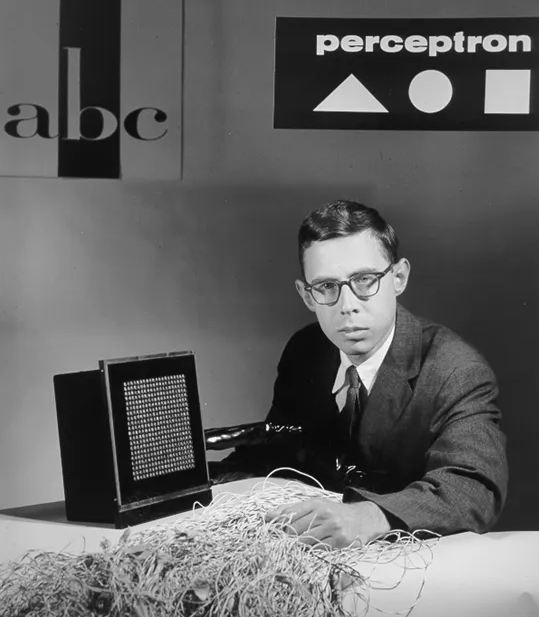
\includegraphics[width=0.95\textwidth]{./images/people/rosenblat_1.png}\\
            {\tiny 
            Rosenblatt and a part of his perceptron.\\
            \color{col:attribution} 
            Image reproduced from \cite{AIPlainEng:RiseAndFallOfPerceptron}\\}
         \end{center}
        \end{column}
        \begin{column}{0.65\textwidth}
            \begin{center}
                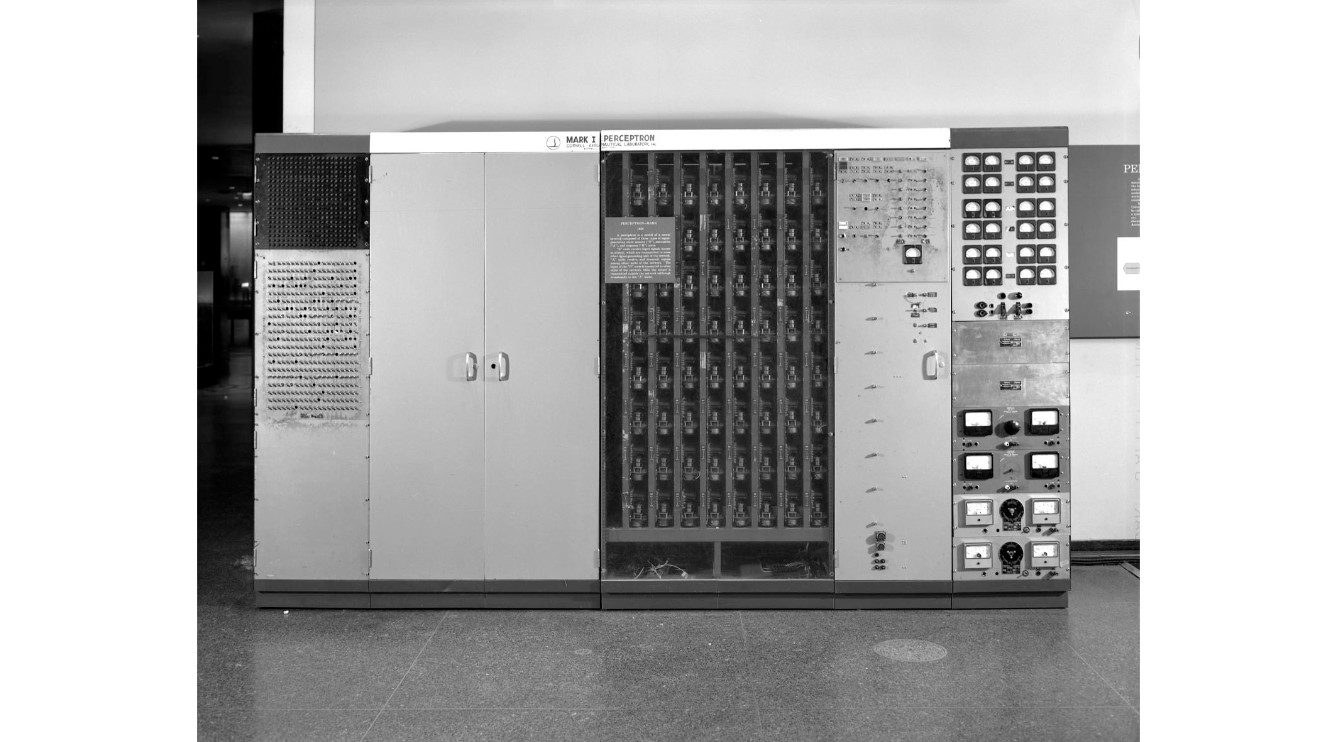
\includegraphics[width=0.98\textwidth]{./images/perceptron/mark1.png}\\
                {\tiny 
                The Mark 1 perceptron.\\
                \color{col:attribution} 
                Courtesy of The Smithsonian Institute\\ (Source: National Museum of American History)\\}
             \end{center}
        \end{column}
      \end{columns}
\end{frame}
